\section{Time Dissection of a Software Update}
We have seen that the lifecycle of a software update comprises four distinct phases\footnote{For a detailed description of each phase the interested reader should read the corresponding paper.} depicted in figure \ref{lifecycle}.

\begin{figure}[h!]
    \caption{The lifecycle of a software update (a decentralized approach)}
    \centering
    \includegraphics[width=\textwidth]{../../figures/lifecycle_phases.pdf}
   % \includegraphics[width=1.0 \columnwidth,keepaspectratio]{figures/lifecycle_phases.pdf}
    \label{lifecycle}
\end{figure}


\subsection{The Ideation Phase}
Let us take as an example the ideation phase and try to dissect the elapsed time. The ideation phase is depicted in figure \ref{ideation}. For simplicity, we omit altogether the delegation process and assume that each stakeholder votes for his/her own stake.

\begin{figure}[h!]
    \caption{The ideation phase.}
    \centering
    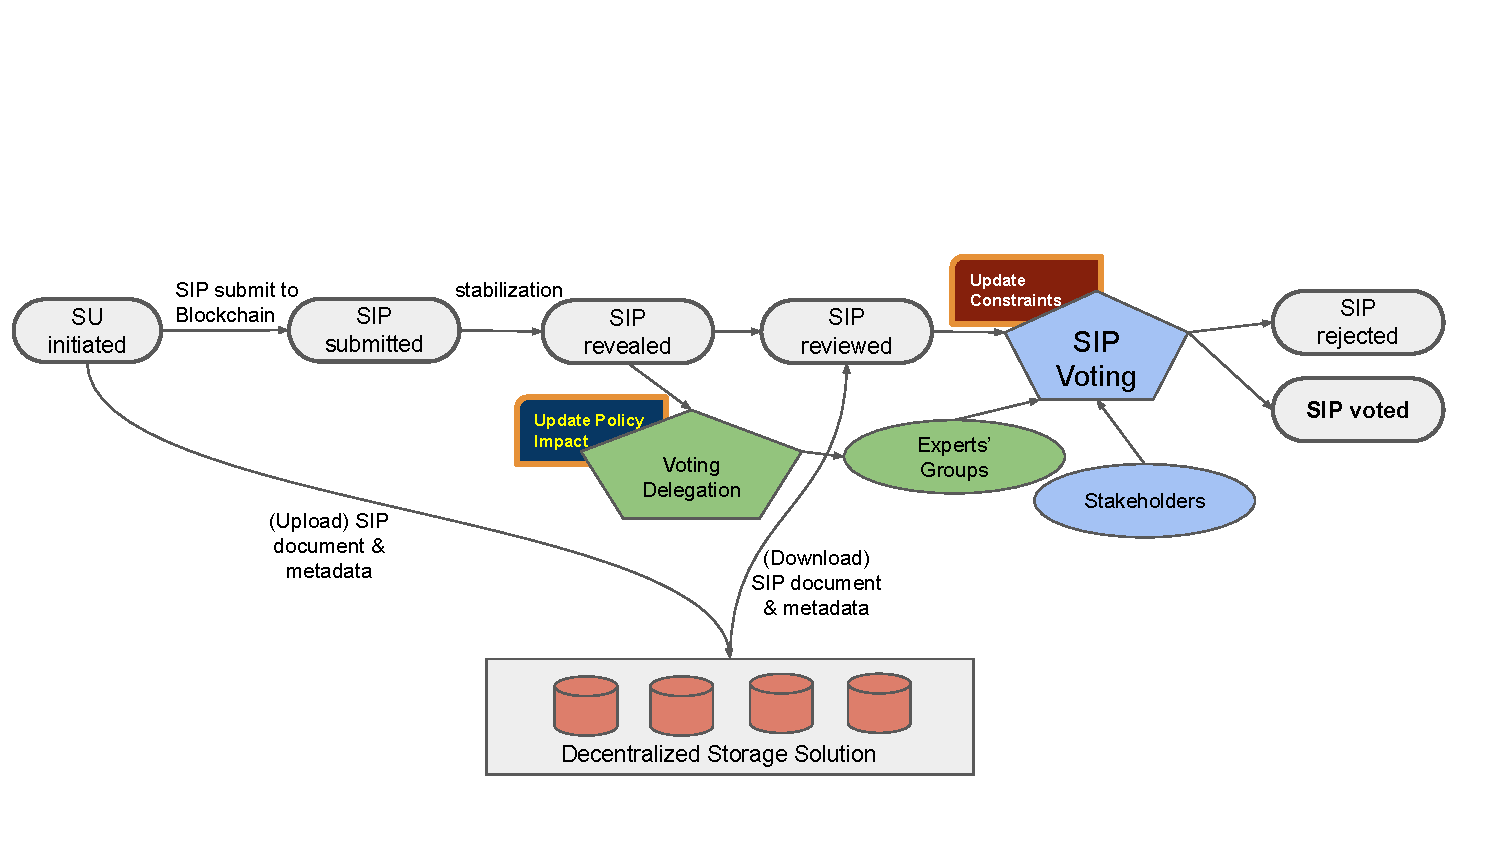
\includegraphics[width=1.0 \columnwidth,keepaspectratio]{../../figures/ideation_phase.pdf}
    \label{ideation}
\end{figure}

\begin{table} [h!]
\centering
%\begin{tabular} {||c | c | l | l | l | l | l ||}
\begin{tabu} to 1.0\textwidth {||X[c] | X[c] | X[l] | X[l] | X[l] | X[l] | X[l] ||}
\hline
\textbf{STEP} & SIP Submitted & SIP Revealed & SIP Reviewed & Upd Constraints Eval & Voting & Tallying \\
\hline
\hline
\textbf{TIME} & $est(u)$ & $est(u)$ & Fixed (i.e., parameter), or a function of SU size & Depends on number of open SUs & Fixed (i.e., parameter), or a function of SU size + $stable(k)$ & Depends on number of votes, which depends on number of users $u$ \\
\hline 
\textbf{METHOD} & Shelley measurements & Shelley measurements & Fixed & Simulation & Fixed & Simulation \\
\hline
\end{tabu}
%\end{tabular}
\caption{Software update time dissection in the ideation phase.}
\label{ideation_dis}
\end{table}

In table \ref{ideation_dis}, we record the \emph{sequential steps} that a software update (SU) goes through in the ideation phase. The first two steps (SIP submitted and SIP revealed) include the time for submitting to the network two separate transactions based on a commit-reveal scheme. The former is the submission of the SIP in an encrypted form and the latter is the submission of the SIP unencrypted. The time required to perform each one of these steps ($est$), is the time required for the submission of an event (\emph{Event Submission Time})to the network and we assume that will be provided by the Shelley measurements. For more details read the corresponding Section \ref{shelley} (Shelley Prerequisites).

\paragraph{SIP reviewed.} The ''SIP Reviewed'' step is a time period given for review of a SIP. This depends on the size of the SIP (the greater the size the more time must be given for review). The size of a SU is declared in the metadata of the SIP and can be measured in estimated mandays to be implemented. To simplify things, we could consider three distinct sizes of SUs (small, medium and large), which correspond to three distinct fixed time periods for the review phase. Of course, we could just have a single flat fixed period of time for reviewing for all SIPs.

\paragraph{Update constraint evaluation.} We currently limit our scope only in two types of update constraints: a) Conflict resolution and b) dependency check. For the former, we want to search the list of open SUs and check if the current SU impacts the same protocol parameters with some other \emph{open SU}\footnote{An \emph{open} SU is a software update that is still competing with other SUs to get approved and become activated.}. In that case, if both belong to the same  phase then are both rejected, otherwise the one in the earlier phase is rejected only. In the dependency check case, we just need to check if the declared required version (in the metadata of a SU) is the current version, or a previous version of the system. If it is not, then the SU is rejected as infeasible, since it depends on a version that does not exist(at least yet). So the cost for evaluating the update constraints is linear to the number of open SUs.

\paragraph{Voting.} The voting period in the simplest form is a flat fixed time period, which could be determined by a protocol parameter. If we want to elaborate it, we could say that it depends on the size of SU (the bigger the SU, the longer it takes to the community to decide). Again, like in the review step above, we could define three distinct voting periods corresponding to three distinct sizes of SUs (small, medium and large). Also, we need to consider a $stable(k)$ period of time, following at the end of the voting period, in order for all the votes to be stably committed to the blockchain.

\paragraph{Tallying.} This is indeed the most complicated step to measure. The tallying step starts immediately after the stabilization period following the voting period and it roughly comprises the following steps: 
\begin{itemize}
\item Search for vote transactions in a specific slot window (the SU's voting period)
\item For each voter's key get the last vote only (ignore the previous ones).
\item For the voter's key on the selected vote find the corresponding stake (We assume that the stake distribution is computed and kept as a local state).
\item  Sum the total stake from the gathered votes.
\end{itemize}
This process depends on the number of votes (i.e., transactions) committed to the blockchain within the voting period window. The number of votes is directly depended on the number of users $u$ participating in the protocol. %Of course, we could maintain the vote result as a local state (a result aggregate per SU) and aggregate the votes as they arrive from the network, in parallel to the voting period. 
Note that the voting result might trigger a new voting period for an SU (in the case of no-quorum and no-majority).

\subsection{The Implementation Phase}
In figure \ref{implementation} we depict the implementation phase.

\begin{figure}[h!]
    \caption{The implementation phase.}
    \centering
    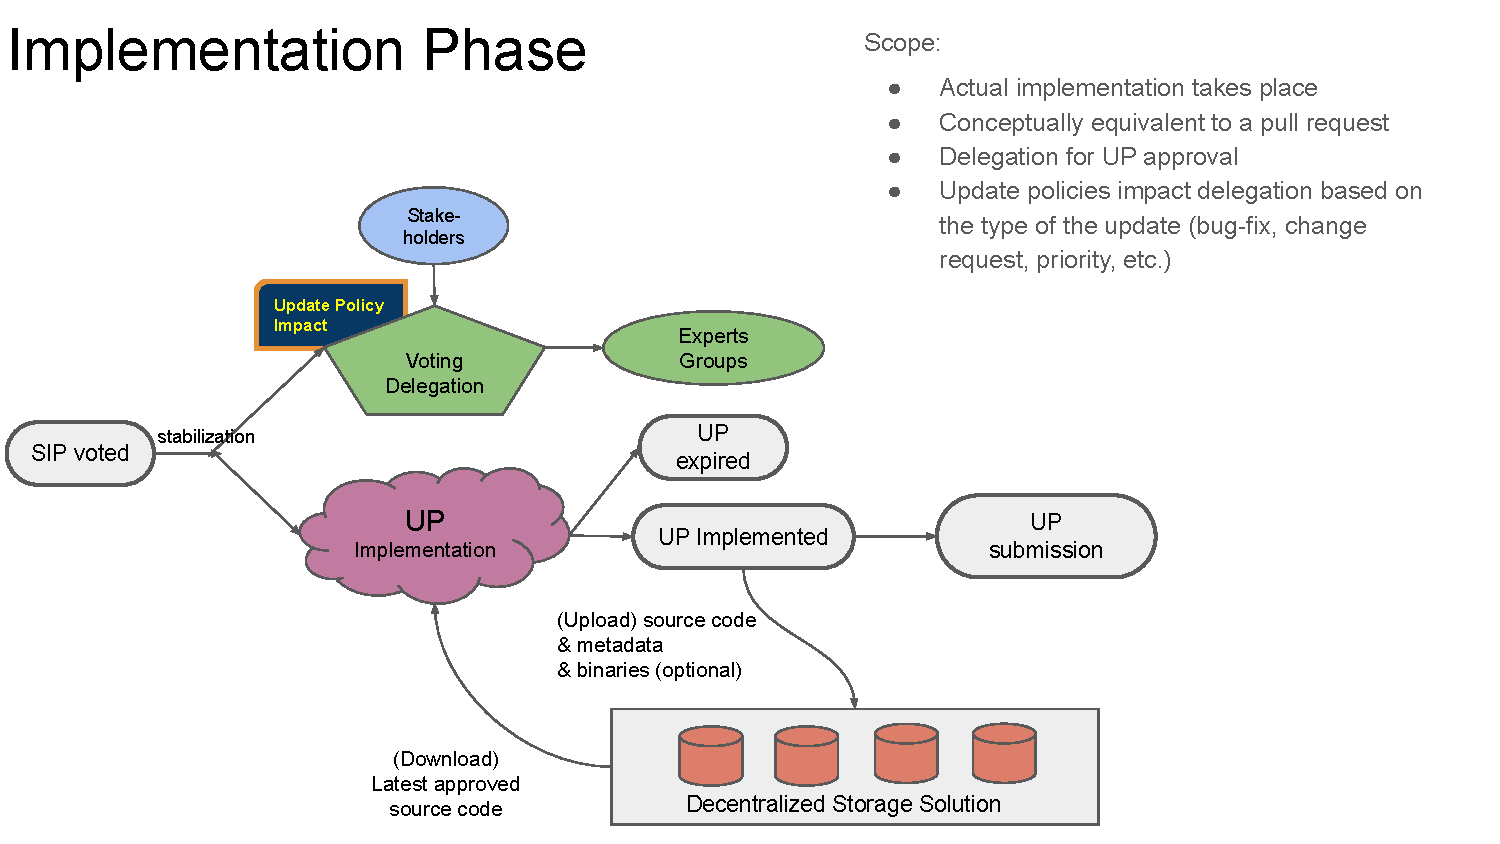
\includegraphics[width=1.0 \columnwidth,keepaspectratio]{../../figures/implementation_phase.pdf}
    \label{implementation}
\end{figure}

In table \ref{implementation_dis}, we summarize the time dissection of a software update in the implementation phase.

\begin{table} [h!]
\centering
%\begin{tabular} {||c | c | l | l | l | l | l ||}
\begin{tabu} to 1.0\textwidth {||X[c] | X[l] | X[c]||}
\hline
\textbf{STEP} & UP Implementation & UP Submission\\
\hline
\hline
\textbf{TIME} & Fixed (i.e., parameter), or a function of SU size & $est(u)$ \\
\hline 
\textbf{METHOD} & Fixed & Shelley measurements \\
\hline
\end{tabu}
%\end{tabular}
\caption{Software update time dissection in the implementation phase.}
\label{implementation_dis}
\end{table}


\subsection{The Approval Phase}
In figure \ref{approval} we depict the approval phase.

\begin{figure}[h!]
    \caption{The approval phase.}
    \centering
    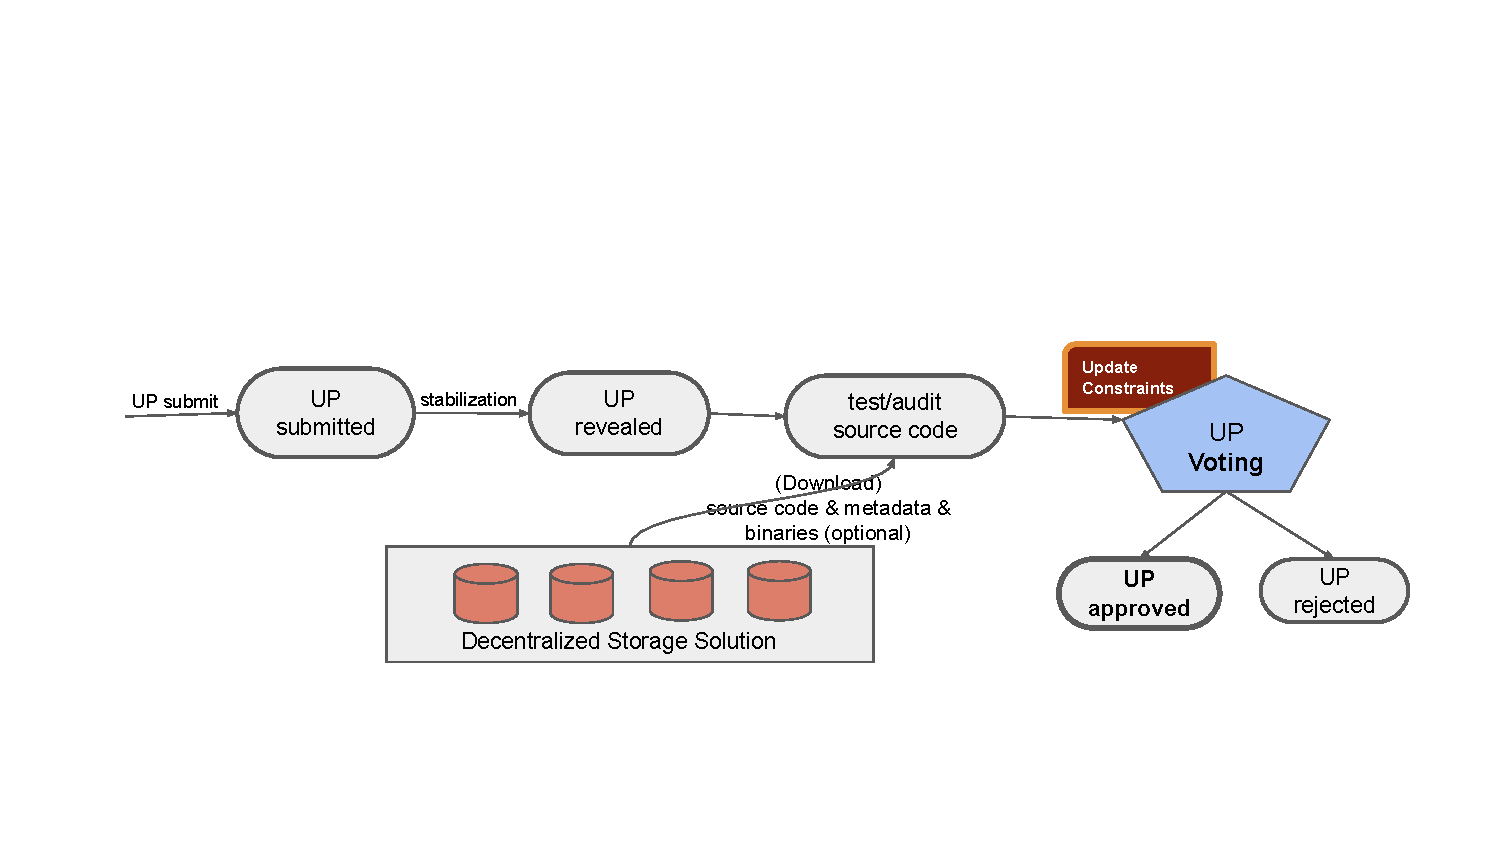
\includegraphics[width=1.0 \columnwidth,keepaspectratio]{../../figures/approval_phase.pdf}
    \label{approval}
\end{figure}

In table \ref{approval_dis}, we summarize the time dissection of a software update in the approval phase. We see that it is essentially identical to the ideation phase.

\begin{table} [h!]
\centering
%\begin{tabular} {||c | c | l | l | l | l | l ||}
\begin{tabu} to 1.0\textwidth {||X[c] | X[c] | X[l] | X[l] | X[l] | X[l] | X[l] ||}
\hline
\textbf{STEP} & UP Submitted & UP Revealed & UP Reviewed & Upd Constraints Eval & Voting & Tallying \\
\hline
\hline
\textbf{TIME} & $est(u)$ & $est(u)$ & Fixed (i.e., parameter), or a function of SU size & Depends on number of open SUs & Fixed (i.e., parameter), or a function of SU size + $stable(k)$ & Depends on number of votes, which depends on number of users $u$ \\
\hline 
\textbf{METHOD} & Shelley measurements & Shelley measurements & Fixed & Simulation & Fixed & Simulation \\
\hline
\end{tabu}
%\end{tabular}
\caption{Software update time dissection in the approval phase.}
\label{approval_dis}
\end{table}


\subsection{The Activation Phase}

In figure \ref{activation} we depict the activation phase.

\begin{figure}[h!]
    \caption{The activation phase.}
    \centering
    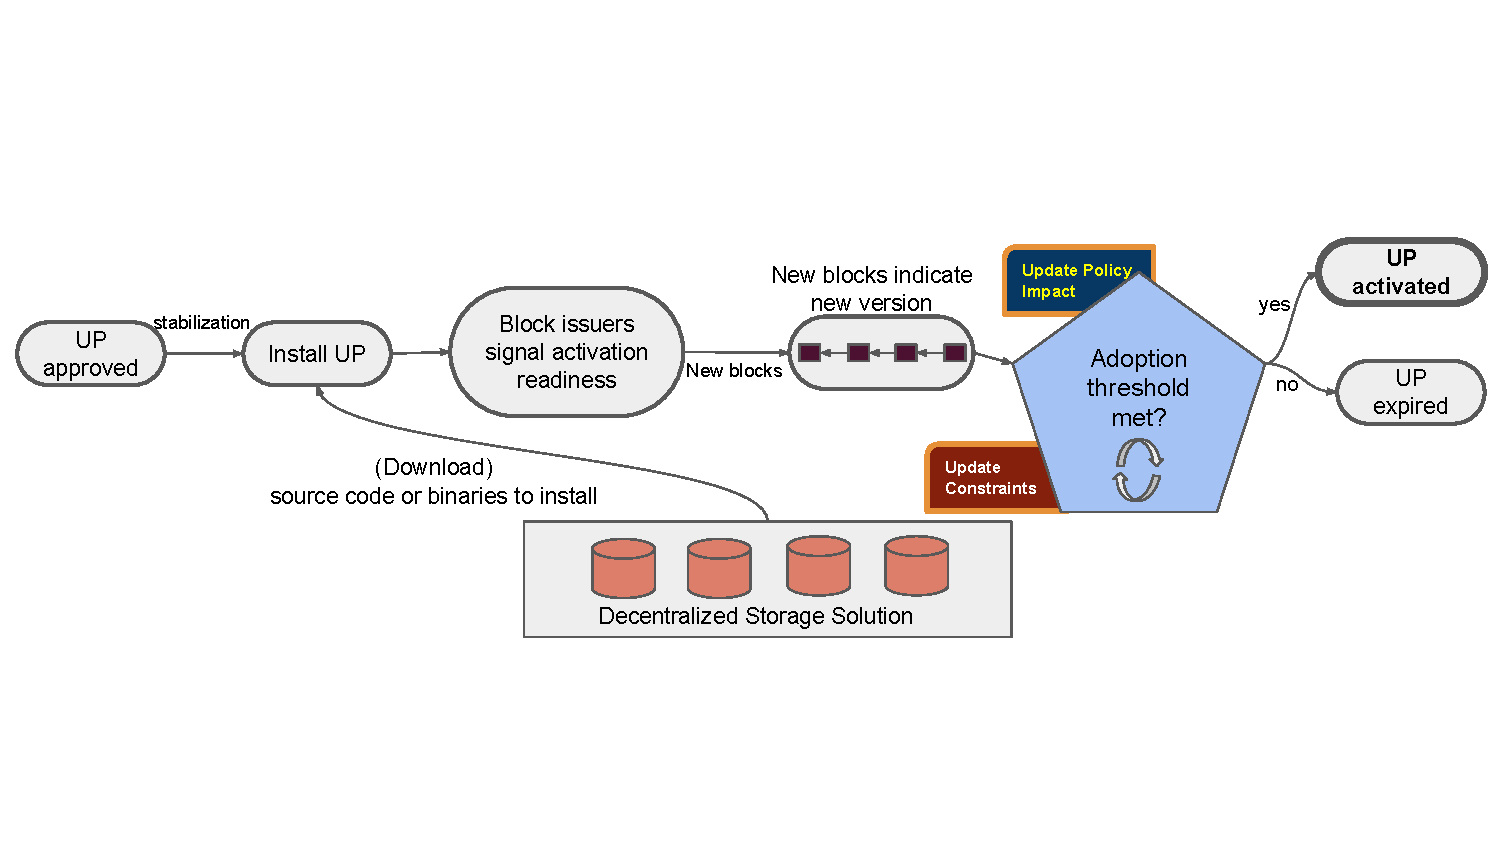
\includegraphics[width=1.0 \columnwidth,keepaspectratio]{../../figures/activation_phase.pdf}
    \label{activation}
\end{figure}

In table \ref{activation_dis}, we summarize the time dissection of a software update in the activation phase. 

\begin{table} [h!]
\centering
%\begin{tabular} {||c | c | l | l | l | l | l ||}
\begin{tabu} to 1.0\textwidth {||X[c] | X[l] | X[c] | X[l] | X[l]||}
\hline
\textbf{STEP} & Install UP & Signal Submission & Signal Tallying & Activation Lag\\
\hline
\hline
\textbf{TIME} & Fixed (i.e., parameter), or a function of SU size & $sst(u)$ & Depends on number of signals, which depends on number of users $u$  & Fixed (i.e., parameter), or a function of SU size \\
\hline 
\textbf{METHOD} & Fixed & Shelley measurements & Simulation & Fixed \\
\hline
\end{tabu}
%\end{tabular}
\caption{Software update time dissection in the activation phase.}
\label{activation_dis}
\end{table}